\documentclass[12pt,a4paper]{article}

% Margins.
\setlength{\oddsidemargin}{0in}
\setlength{\evensidemargin}{0in}
\setlength{\headheight}{12pt}
\setlength{\headsep}{0pt}
\setlength{\topmargin}{-60pt}
\setlength{\textwidth}{6.5in}
\setlength{\textheight}{10.75in}

\usepackage{amsmath}
\usepackage{float}
\usepackage{graphicx}
\usepackage[hyphens]{url}
\usepackage{hyperref}	% Clickable links to figures, references and urls.
\usepackage{datetime}
\usepackage{longtable}

% Links direct to top of figures.
\usepackage[all]{hypcap}

% Drawing.
\usepackage{pgf}
\usepackage{tikz}

% Listings for formatting code.
\usepackage{listings}
\usepackage{textcomp}
% General options.
\lstset{breaklines=true, basicstyle=\small\ttfamily, tabsize=4, numbers=left, stepnumber=1, frame=single, showstringspaces=false, upquote=true}
% C++ specific high-lighting. Comments are 50/50 shades of green/black and strings coloured with 60/40 red/black mixture.
\lstset{language=[ISO]C++, commentstyle=\color{green!50!black}, keywordstyle=\color{blue}, stringstyle=\color{red!60!black}}

%opening
\title{Electromagnetic Theory\\Class 06\\Vector Transformations}
\author{Attique Dawood}
\date{September 05, 2014\\[0.2cm] Last Modified: \today, \currenttime}
\begin{document}
\maketitle
\section{Announcements}
\begin{itemize}
\item None.
\end{itemize}
\section{Revision}
\begin{itemize}
\item Curvilinear coordinate systems.
\end{itemize}
\section{Unit Vector Transformations Between Cartesian and Cylindrical Coordinates}
A vector \textbf{A} in Cartesian and Cylindrical coordinates is expressed in terms of the respective unit vectors. That is,
\begin{equation}
\textbf{A}=A_x\hat x+A_y+\hat y+A_z\hat z=A_{\rho}\hat \rho+A_{\phi}\hat \phi+A_z\hat z
\end{equation}
An extensive discussion on how vectors transform between different coordinate systems is not a part of this course but here we discuss unit vector transformation between cylindrical and spherical coordinate systems. Please consult the reference book \cite[Chapter 2]{Sadiku} for a detailed discussion on vector transformation.

Suppose we want to express vectors $\hat x$ and $\hat y$ in cylindrical coordinates and vice versa. By referring to figure \ref{Cylindrical-Spherical-transformation} taken from ~\cite[Figure 2.3, page 31]{Sadiku} the transformation are
\begin{equation}
\begin{split}
&\hat x=\cos\phi\hat \rho-\sin\phi \hat \phi\\
&\hat y=\sin\phi\hat \rho+\cos\phi \hat \phi\\
&\hat z=\hat z
\end{split}
\end{equation}
\begin{equation}
\begin{split}
&\hat \rho=\cos\phi\hat x+\sin\phi \hat y\\
&\hat \phi=-\sin\phi\hat x+\cos\phi \hat y\\
&\hat z=\hat z
\end{split}
\end{equation}
\begin{figure}[H]
\centering
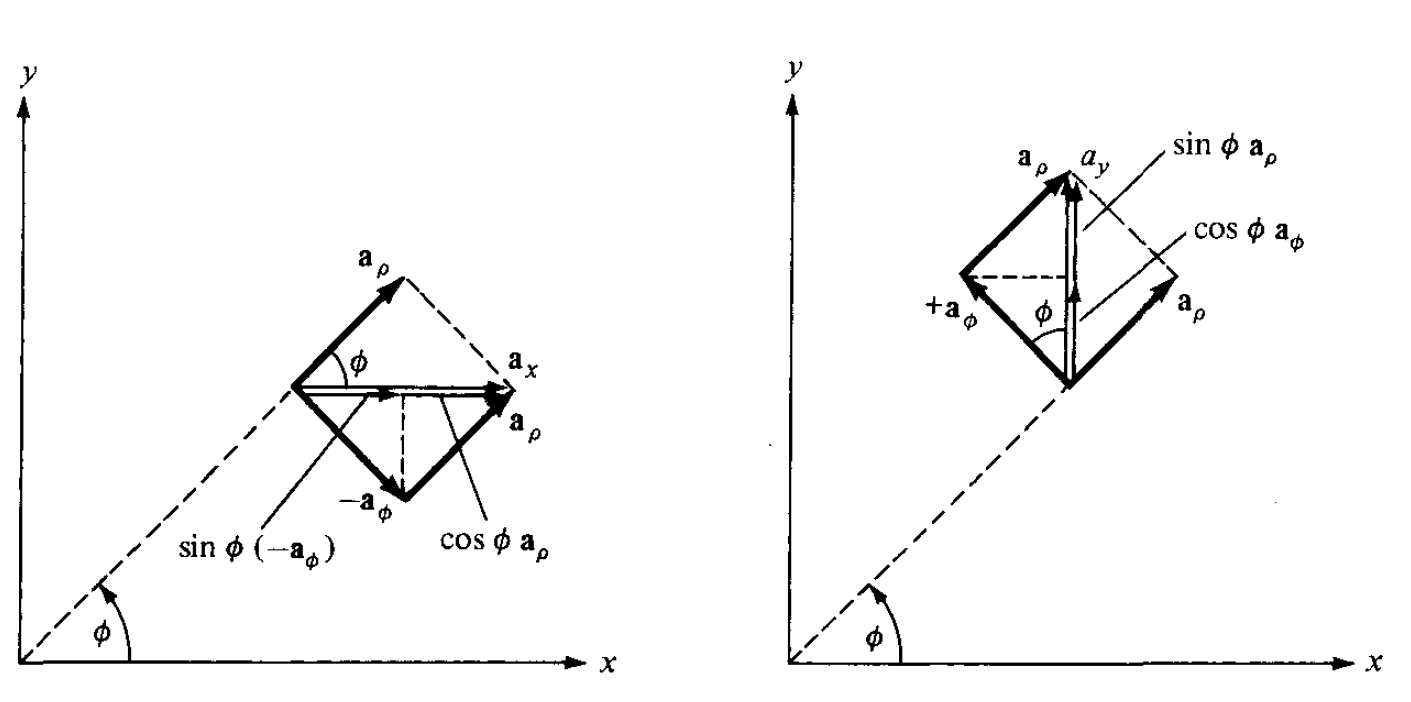
\includegraphics[scale=0.4]{Figure2-3S.png}
\caption{Unit vector transformations. Figure taken from~\cite[Figure 2.3, page 31]{Sadiku}}
\label{Cylindrical-Spherical-transformation}
\end{figure}
\section{Exercises}
\noindent\textbf{Question 1:}
\begin{itemize}
\item[(1)] Convert points P(1, 3, 5) T(0, -4, 3) and S(-3, -4, -10) to cylindrical and spherical coordinates.
\item[(2)] Transform \textbf{A}$=\hat x$ to cylindrical and spherical coordinates.
\item[(3)] Calculate \textbf{A} at T in cylindrical and spherical coordinates.
\end{itemize}
%\nocite{*}
\bibliographystyle{plain}
\bibliography{EMTRef}
\end{document}
